\documentclass[aspectratio=169]{beamer}  
\usefonttheme{professionalfonts}
\usepackage{xeCJK}
\usepackage{fontspec}
\usepackage{graphicx}
\usepackage{listings}
\usepackage{xcolor}
\usepackage{indentfirst}
\usepackage{tikz}
\usepackage{amssymb}
\usepackage{amsthm}
\usepackage{amsmath}
\usepackage{tabularx}
\usepackage{hyperref}
\usepackage{comment}
\usepackage{ulem}
\usepackage{version}
\usepackage{thmtools}
\usepackage{qtree}
\usepackage{algpseudocode}
\usepackage{mathtools}
\usepackage{multicol}
\usepackage{xcolor}
\usepackage{diagbox}

\usefonttheme[onlymath]{serif}

\XeTeXlinebreaklocale "zh"
\XeTeXlinebreakskip = 0pt plus 1pt

\setsansfont{JetBrainsMono-Medium.ttf}
\setCJKmainfont[AutoFakeBold,AutoFakeSlant]{NotoSansTC-Regular.otf}
\usetikzlibrary{arrows,decorations.markings,decorations.pathreplacing}
\newenvironment{Hint}{\noindent\textbf{Hint.}}{}

\tikzstyle {graph node} = [circle, draw, minimum width=1cm]
\tikzset{edge/.style = {decoration={markings,mark=at position 1 with %
            {\arrow[scale=2,>=stealth]{>}}},postaction={decorate}}}

\lstset{
    language=C++,
    basicstyle=\ttfamily\tiny,
    commentstyle=\color{black!50},
    keywordstyle=\color{white!0!blue},
    stringstyle=\color{black!50!green},
    showspaces=false,
    showstringspaces=false,
    showtabs=false,
    tabsize=4,
    captionpos=b,
    breaklines=true,
    breakatwhitespace=false,
    escapeinside={\%*}{*)},
    morekeywords={*}
}

\AtBeginSection[]{
  \begin{frame}
  \vfill
  \centering
  \begin{beamercolorbox}[sep=8pt,center,shadow=true,rounded=true]{title}
    \usebeamerfont{title}\insertsectionhead\par%
  \end{beamercolorbox}
  \vfill
  \end{frame}
}

\title{基礎演算法 III}
\author{sam571128}
\date[附中延平競程讀書會]

\usetheme{Madrid}
\usecolortheme{default}
\setbeamertemplate{itemize items}[square]
\setbeamertemplate{enumerate items}[default]
\setbeamertemplate{blocks}[default]

\begin{document}

    %title
    \begin{frame}
        \titlepage
    \end{frame}
    
    \begin{frame}{小小的自我介紹}
        \begin{itemize}
            \item 常用 handle: sam571128,可以叫我山姆
            \item 我不是附中的學長
            \item 被邪惡的總召騙進來講課了
            \item 跟你們的學長 Foxyy、和 Gino 是高中隊友,隊名 BurnChicken Lemma。 
            \item 聽不懂都可以說,我看到就會回
        \end{itemize}
    \end{frame}
    
    %content
    \begin{frame}{目錄}
        \begin{itemize}
            \item Greedy
            \item 掃描線
            \item 前綴和 \& 差分
            \item 單調隊列
            \item 補充: 模運算
        \end{itemize}
    \end{frame}
    
    \begin{frame}{Greedy}
        \begin{itemize}
            \item 貪心? 什麼是貪心啊?
            \item 讓我們直接來看一個例子
        \end{itemize}
    \end{frame}
    
    \begin{frame}{一個簡單的小例子}
        \begin{block}{找零問題}
            現在,你走進一間商店。你買了 $34$ 塊新台幣的商品。可是你現在身上只有 $100$ 紙鈔。那店員在找零錢的時候,最少要拿幾個硬幣給你?
        \end{block}
        \begin{itemize}
            \item 對於這個問題,你應該會很直接的想到答案
            \item<2-> 首先我們知道店員一共要找我們 $66$ 塊錢
            \item<2-> 接著,你很直覺的就會想到,店員會找 $50 + 10 + 5 + 1$ 給我們
            \item<3-> 而事實上,最少的拿法,就是從最大面額的硬幣開始拿取
        \end{itemize}
    \end{frame}
    
    \begin{frame}{Greedy}
        \begin{itemize}
            \item 從剛剛那個例子當中,我們看到了什麼?
            \item<2-> 事實上,我們照著直覺走,認為只要從最大的硬幣開始選,一定可以選到最少的
            \item<2-> 而這樣的方式,就是 Greedy
        \end{itemize}
    \end{frame}
    
    \begin{frame}{Greedy}
        \begin{itemize}
            \item Greedy 其實就是照著某個策略走,他或許就可以給我們一個正確的答案
            \item 可以把他想成一棵暴搜的樹上,直接照著某個路徑走到正確的答案
        \end{itemize}
        \begin{center}
            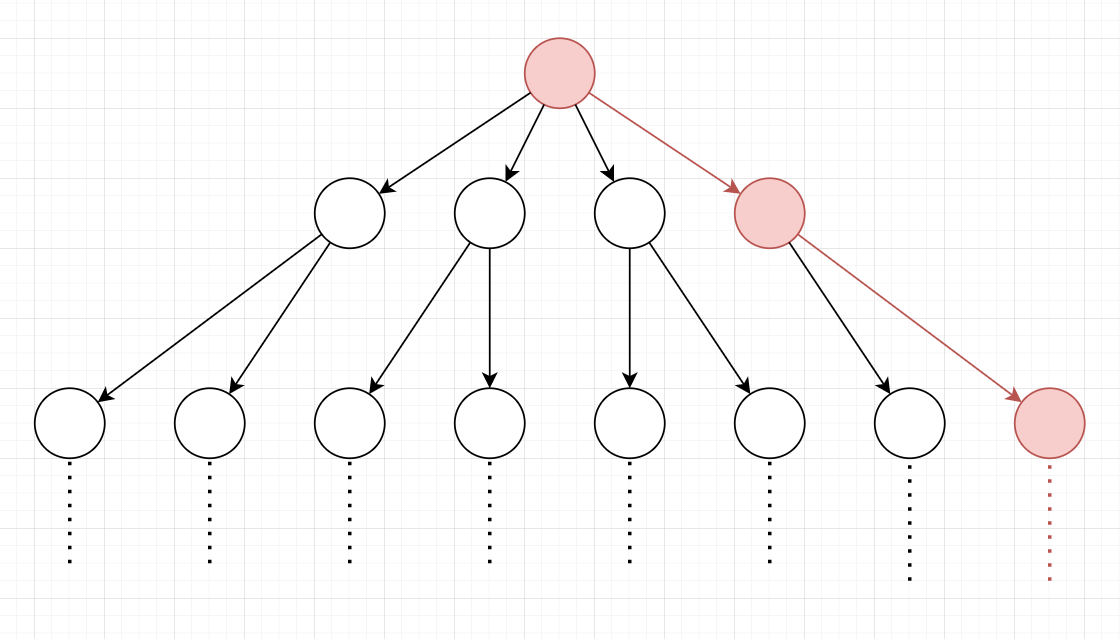
\includegraphics[scale=0.35]{images/greedy_tree.png}
        \end{center}
    \end{frame}
    
    \begin{frame}{Greedy}
        \begin{itemize}
            \item 在很多的情況下,Greedy 的想法還滿直覺的
            \item 像剛剛的硬幣問題,事實上直覺的做法就是正確的方法
            \item 不過並不是任何時候,按照直覺都會讓我們得到正確的答案
        \end{itemize}
    \end{frame}
    
    \begin{frame}{一個貪心會錯的小例子}
        \begin{block}{找零問題 (改)}
            現在,你到了長頸鹿國,這裡的硬幣面額只有 $1, 5, 8$ 塊錢三種種類。你走進一間商店。你買了 $15$ 塊長頸鹿幣的商品。請問你最少要拿出多少硬幣才能購買這個商品。
        \end{block}
        \begin{itemize}
            \item 以這個例子來看的話,使用剛剛的想法,一路拿最大面額的硬幣會發生什麼事?
            \item<2-> 我們會選 $\{8,5,1,1\}$
            \item<3-> 但事實上,你會發現 $\{5,5,5\}$ 才會是最大的答案!
        \end{itemize}
    \end{frame}
    
    \begin{frame}{直覺不見得會是對的?}
        \begin{itemize}
            \item 從剛剛的例子,我們發現到,Greedy 有可能會是錯的
            \item 有時,我們必須要實際去證明 Greedy 的策略後,才能確定他會是對的
            \item<2-> 不過你應該很好奇,同樣都是硬幣,為什麼一個會對一個會錯呢?
        \end{itemize}
    \end{frame}
    
    \begin{frame}{回到剛剛的兩個例子}
        \begin{itemize}
            \item 在第一個例子中,我們所用的是新台幣,面額大概是 $\{1,5,10,50,100,500,1000\}$
            \item 而在第二個例子中,則是使用了面額比較奇怪的硬幣,面額是 $\{1,5,8\}$
            \item 這兩者的差別在哪呢?
            \item<2-> 應該會發現到,第一個例子中,兩兩硬幣互相有因倍數的關係!
            \item<2-> 而這個就會影響到 Greedy 策略的正確性!
        \end{itemize}
    \end{frame}
    
    \begin{frame}{回到剛剛的兩個例子}
        \begin{itemize}
            \item 在這裡,我們來仔細想想看為什麼第一種就會是正確的吧
            \item<2-> 會發現,硬幣互相有倍數關係時,其實我們可以發現,當小面額的數量過多可以被替換成大面額的硬幣時,我們就替換
            \item<2-> 一路將小面額的硬幣替換成大面額後,我們就會得到最少的選法了
            \item<3-> 當然,這個有更加嚴謹的證明寫法
        \end{itemize}
    \end{frame}
    
    \begin{frame}{讓我們來看看下一個例子}
        \begin{block}{\href{https://cses.fi/problemset/task/1629}{活動排程問題 (CSES - Movie Festival)}}
            現在一共有 $n$ 部電影,每部電影的播放時段為 $[l_i, r_i]$。在同一個時間,你只能看一部電影,你希望每一部電影你都能完整看完,請問你最多可以看幾部電影?
        \end{block}
        \begin{itemize}
            \item<2-> 一個滿直覺的想法,既然想要看最多的電影,那從開始時間最早的電影開始看?
            \item<2-> 然後就發現出現問題了
        \end{itemize}
    \end{frame}
    
    \begin{frame}{會發生的問題}
        \begin{itemize}
            \item 注意到當有其中一部電影的開始時間很早,但時長很長
            \item 它就會影響到後面可以看電影的時間
        \end{itemize}
        \begin{center}
            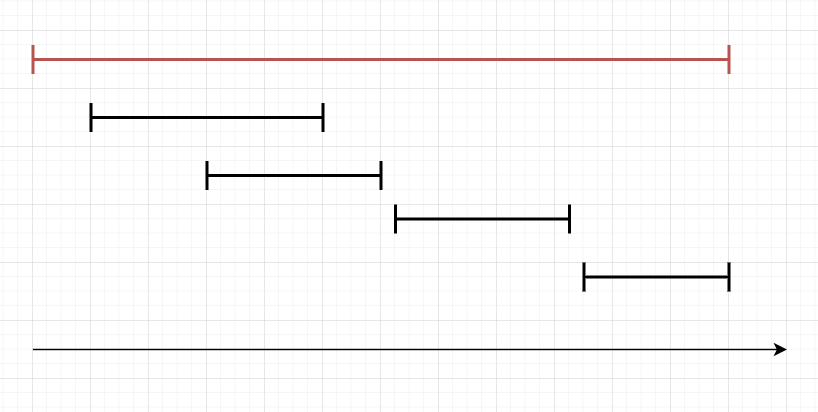
\includegraphics[scale=0.5]{images/movie_festival.png}
        \end{center}
    \end{frame}
    
    \begin{frame}{那該怎麼辦?}
        \begin{itemize}
            \item 既然剛剛的想法是錯的,那我們換一個思路
            \item 一部電影的結束時間越早,是不是就能給我們更多的時間能夠看接下來的電影呢?
        \end{itemize}
    \end{frame}
    
    \begin{frame}{新的想法}
        \begin{center}
            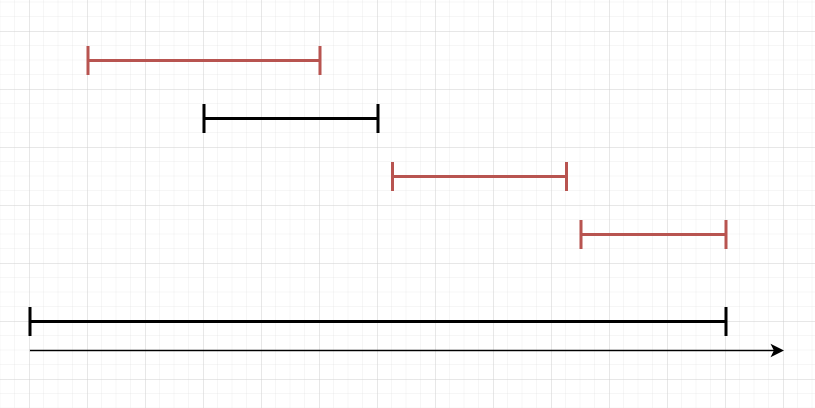
\includegraphics[scale=0.5]{images/movie_festival_2.png}
        \end{center}
        \begin{itemize}
            \item<2-> 這樣的想法,其實是正確的!
        \end{itemize}
    \end{frame}
    
    \begin{frame}{貪心的正確性?}
        \begin{itemize}
            \item 聽到這裡,你可能會覺得,貪心到底是在做什麼
            \item 為什麼我們幾乎都在猜答案?
            \item<2-> 貪心難道就只是單純的猜答案,然後祈禱它會是對的嗎?
        \end{itemize}
    \end{frame}
    
    \begin{frame}{貪心的正確性?}
        \begin{itemize}
            \item 常見的做法:
                \begin{itemize}
                    \item \sout{Proof By AC} (不嚴謹)
                    \item 試著想反例,想不到就丟 (不嚴謹)
                    \item 實際寫下數學證明 (嚴謹)
                \end{itemize}
            \item<2-> 有時候實際證明自己的作法,可能比較不會在比賽中去做
            \item<2-> 但學習如何證明貪心的做法也算是一個重要的能力
        \end{itemize}
    \end{frame}
    
    \begin{frame}{簡單證明一下剛剛的活動排程問題}
        \begin{enumerate}
            \item 設貪心所拿的線段為 $\{a_1,a_2,\dots,a_n\}$,而一種最佳解所取的線段為 $\{b_1,b_2,\dots,b_m\}$
            \item 可以得知,對於所有 $i \le n$,$r_{a_i}$ 必定小於 $r_{b_i}$,可以使用數學歸納法簡單證明
            \item 接著,假設貪心所拿的線段比最佳解還少,表示最佳解至少比貪心多拿了一個線段
            \item 但由於 $r_{a_n} \le r_{b_i} \le l_{b_{i+1}}$,貪心解一定也可以取第 $b_i$ 條線段
            \item 產生矛盾。因此貪心解一定會取到最多的線段。
        \end{enumerate}
    \end{frame}
    
    \begin{frame}{下一個例題}
        \begin{block}{\href{https://tioj.ck.tp.edu.tw/problems/1072}{TIOJ 1072 誰先晚餐}}
            有 $n$ 個人來餐廳吃飯,第 $i$ 個人點的餐點要花 $c_i$ 分鐘煮,煮完後他要吃 $e_i$ 分鐘。廚師在同一個時間只
            能煮一個人的菜,但大家可以同時吃飯,至少要花多少時間才能讓所有人吃完飯。
        \end{block}
        \begin{itemize}
            \item<2-> 既然要讓每個人吃完飯的時間最短,那我們讓煮最久的餐點先煮呢?
        \end{itemize}
    \end{frame}
    
    \begin{frame}{誰先晚餐}
        \begin{itemize}
            \item 會發現,這樣的想法並不會是最好的,可以很輕易的構出更好的解
        \end{itemize}
        \begin{center}
            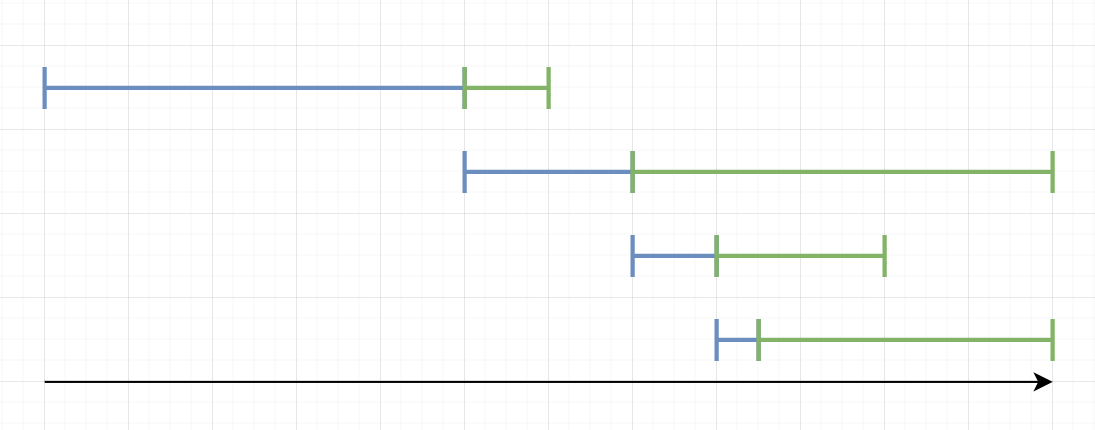
\includegraphics[scale=0.5]{images/who_dinner_first.png}
        \end{center}
    \end{frame}
    
    \begin{frame}{誰先晚餐}
        \begin{itemize}
            \item 剛剛的想法,在某個人的餐點準備時間很短,但吃很慢的時候會發生問題
            \item<2-> 那我們修改策略,讓吃比較慢的人先吃呢?
        \end{itemize}
    \end{frame}
    
    \begin{frame}{誰先晚餐}
        \begin{itemize}
            \item 事實上,這樣的做法就是對的了!
        \end{itemize}
        \begin{center}
            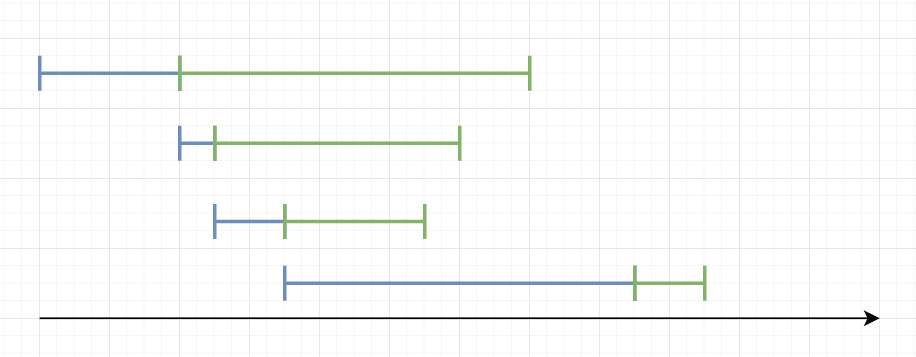
\includegraphics[scale=0.5]{images/who_dinner_first_2.png}
        \end{center}
    \end{frame}
    
    \begin{frame}{誰先晚餐 證明}
        \begin{enumerate}
            \item 首先,我們設貪心解的順序為 $a_1, a_2, \cdots, a_n$,一定滿足 $e_{a_1} \ge e_{a_2} \ge \cdots \ge e_{a_n}$
            \item 而另一組解的順序為 $b_1, b_2, \cdots, b_n$,而這個順序一定存在一個 $i$,使得 $e_{b_i} < e_{b_{i+1}}$
            \item 發現到對於另一組解所得到的順序中,第 $j$ 個人吃完飯的時間為 $(\sum_{k=1}^j C_{b_k}) + E_{b_j}$
            \item 假設我們將第一個使得 $e_{b_i} < e_{b_{i+1}}$ 的 $b_i$ 與 $b_{i+1}$ 進行對調
            \item 第 $i$ 個人吃完飯的時間變為 $(\sum_{k=1}^i C_{b_k}) - C_{b_i} + C_{b_{i+1}} + E_{i+1}$
            \item 第 $i+1$ 個人吃完飯的時間變為 $(\sum_{k=1}^i C_{b_k}) + E_{i}$
            \item 而不論是第 $i$ 或第 $i+1$ 個人,吃完飯的時間都比原本的第 $i+1$ 個人還要早吃完,答案不會變差
            \item 因此只要不停交換使得 $e_{b_i} < e_{b_{i+1}}$ 的 $b_i, b_{i+1}$,最後就會得到貪心所得到的解
        \end{enumerate}
    \end{frame}
    
    \begin{frame}{經典例題(一)}
        \begin{block}{\href{https://cses.fi/problemset/task/1161}{CSES - Stick Division}}
            現在你有一個長度為 $x$ 的木棒,你希望可以將其切成長度為 $a_1, a_2, \cdots, a_n$ 的部分。每一次在切的時候,你會需要耗費當前木棒長度的能量。請問你最少要耗費多少能量才可以切割完這個木棒。
        \end{block}
        \begin{itemize}
            \item<2-> 發現到切割其實等同於將兩個大小為 $x,y$ 的部分合併,耗費 $x+y$ 的能量
            \item<3-> 我們可以將目前的所有木棒丟進一個 priority\_queue,每次拿出最小的兩個木棒進行合併。
        \end{itemize}
    \end{frame}
    
    \begin{frame}{經典例題(二)}
        \begin{block}{\href{https://codeforces.com/problemset/problem/1526/C2}{Codeforces 1526C2 - Potions (Hard Version)}}
            在數線上依序擺著 $n$ 瓶藥水,喝完藥水後,你的血量會改變 $a_i$ (正的表示補血,負的會扣血)。你一開始的血量為 $0$,必須依序從左走到右,每個藥水可喝可不喝,但是喝完之後,血量不能低於 $0$。請問你最多可以喝幾瓶藥水?
        \end{block}
        \begin{itemize}
            \item<2-> 對於藥水,我們其實可以分為補血和扣血的兩個進行考慮
            \item<3-> 當我們遇到補血藥水時,喝掉一定不會比較差
            \item<4-> 那扣血藥水呢?
        \end{itemize}
    \end{frame}
    
    \begin{frame}{經典例題(二)}
        \begin{block}{\href{https://codeforces.com/problemset/problem/1526/C2}{Codeforces 1526C2 - Potions (Hard Version)}}
            在數線上依序擺著 $n$ 瓶藥水,喝完藥水後,你的血量會改變 $a_i$ (正的表示補血,負的會扣血)。你一開始的血量為 $0$,必須依序從左走到右,每個藥水可喝可不喝,但是喝完之後,血量不能低於 $0$。請問你最多可以喝幾瓶藥水?
        \end{block}
        \begin{itemize}
            \item 如果遇到扣血藥水,有兩種可能性
            \begin{enumerate}
                \item 現在的血量在喝完藥水後,不會小於 $0$
                \item 喝完之後,血量會小於 $0$
            \end{enumerate}
            \item<2-> 顯然遇到第一種 case 的時候,我們直接喝掉就好
            \item<2-> 那第二種呢?
        \end{itemize}
    \end{frame}
    
    \begin{frame}{經典例題(二)}
        \begin{block}{\href{https://codeforces.com/problemset/problem/1526/C2}{Codeforces 1526C2 - Potions (Hard Version)}}
            在數線上依序擺著 $n$ 瓶藥水,喝完藥水後,你的血量會改變 $a_i$ (正的表示補血,負的會扣血)。你一開始的血量為 $0$,必須依序從左走到右,每個藥水可喝可不喝,但是喝完之後,血量不能低於 $0$。請問你最多可以喝幾瓶藥水?
        \end{block}
        \begin{itemize}
            \item 有可能發生的事情是,在前面,我們喝過了扣血的藥水,導致我們現在沒有辦法喝這個藥水
            \item<2-> 把每個喝過的藥水存起來,如果換掉前面喝過的藥水,能夠讓我們喝完這個藥水後,血量還更高,就替換
            \item<3-> 使用一個 pq 存喝過的藥水即可
            \item<4-> 這種將前面操作刪除的 Greedy,我們一般稱其為反悔 Greedy
        \end{itemize}
    \end{frame}
    
    \begin{frame}{經典例題(三)}
        \begin{block}{分數背包問題 (Fractional Knapsack Problem)}
            現在你有一個容量為 $W$ 的背包,桌上有 $n$ 個物品,第 $i$ 個物品的重量為 $w_i$,價值為 $v_i$。對於每個物品,你可以選擇將其放進背包,或者是只拿一部分放進背包。請問你最多可以拿到總價值為多少的物品?
        \end{block}
        \begin{itemize}
            \item<2-> 其實只要從 CP 值 ($\dfrac{v_i}{w_i}$) 最大的物品開始拿即可
        \end{itemize}
    \end{frame}
    
    \begin{frame}{經典例題(四)}
        \begin{block}{字串串接問題 (Codeforces 632C - The Smallest String Concatenation)}
            現在你有 $n$ 個字串,現在你想要把這些字串接在一起,請問能使最後接出來的字串的字典序最小的接法為何?
        \end{block}
        \begin{itemize}
            \item<2-> 有沒有人有什麼 Greedy 的想法呢?
            \item<3-> 實際上,這題只要排序就好!
            \item<4-> 排序的函數為 $a+b < b+a$
        \end{itemize}
    \end{frame}
    
    \section{掃描線 (Sweep Line)}
    
    \begin{frame}{什麼是掃描線?}
        \begin{itemize}
            \item 當我們遇到二維平面上的線段、矩形,甚至是三角形或圓時
            \item 用一條鉛直或水平的線進行處理,問題就會簡化許多
        \end{itemize}
        \begin{center}
            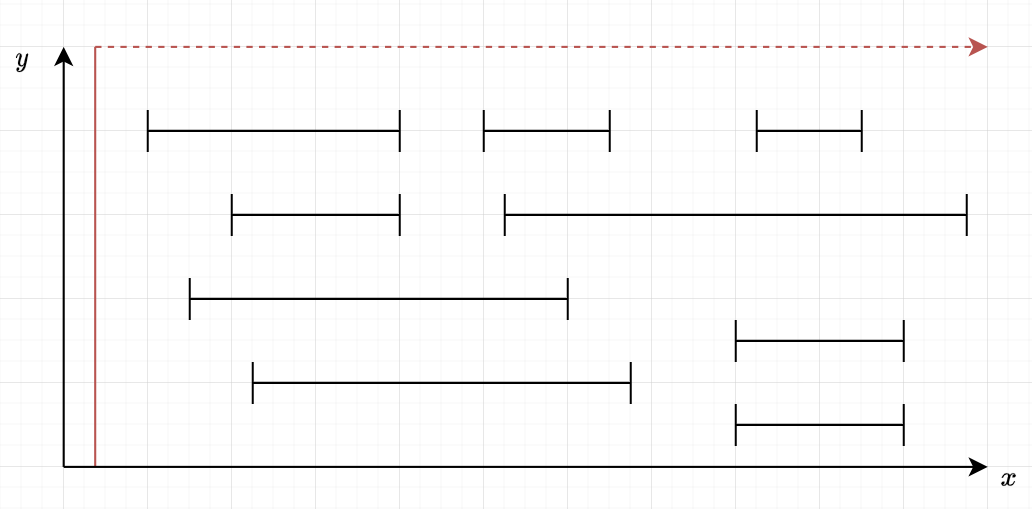
\includegraphics[scale=0.4]{images/sweep_line.png}
        \end{center}
    \end{frame}
    
    \begin{frame}{來看一個簡單的例題}
        \begin{block}{\href{https://zerojudge.tw/ShowProblem?problemid=b966}{線段覆蓋長度 (APCS 2016/03)}}
            給你 $n$ 條線段,每個線段覆蓋了 $[l_i,r_i]$,請找到這些線段一共覆蓋了多少長度? \\
            \vspace{5mm}
            範圍:
            \begin{itemize}
                \item $1 \le n \le 10^4$
                \item $1 \le l_i,r_i \le 10^9$
            \end{itemize}
        \end{block}
        \begin{center}
            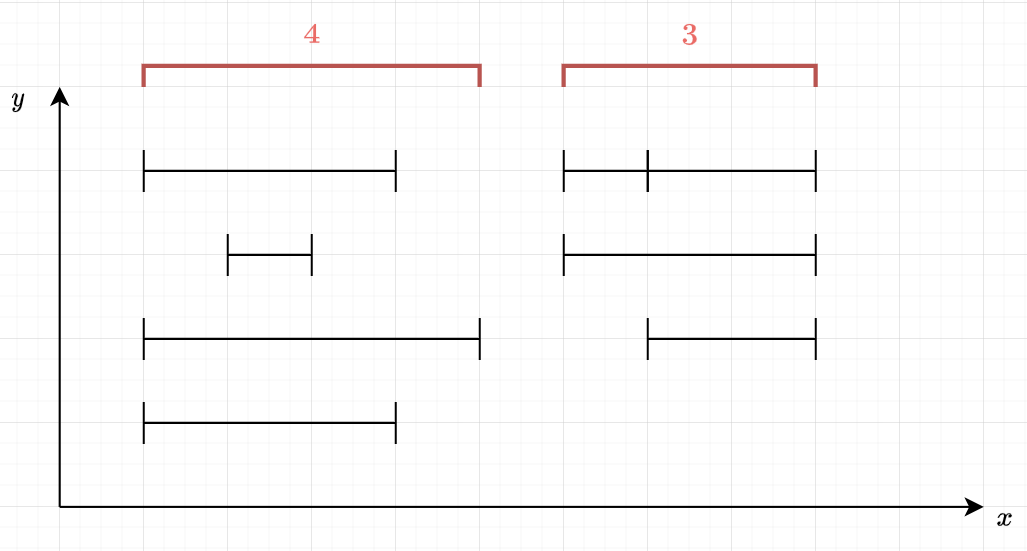
\includegraphics[scale=0.2]{images/segment_union_length.png}
        \end{center}
    \end{frame}
    
    \begin{frame}{線段覆蓋長度}
        \begin{itemize}
            \item 對於這個問題,我們使用掃描線的想法,固定一個鉛直的掃描線,從左掃到右
            \item 只要找到掃描線一共在多少時間有經過線段即可
        \end{itemize}
    \end{frame}
    
    \begin{frame}{線段覆蓋長度}
        \begin{itemize}
            \item 事實上,需要考慮的只有每個線段的端點
            \item 將每條線段的左右界分別考慮,當掃描線掃過左界時,表示掃描線進入線段
            \item 反之經過右界時,表示離開線段
        \end{itemize}
        \begin{center}
            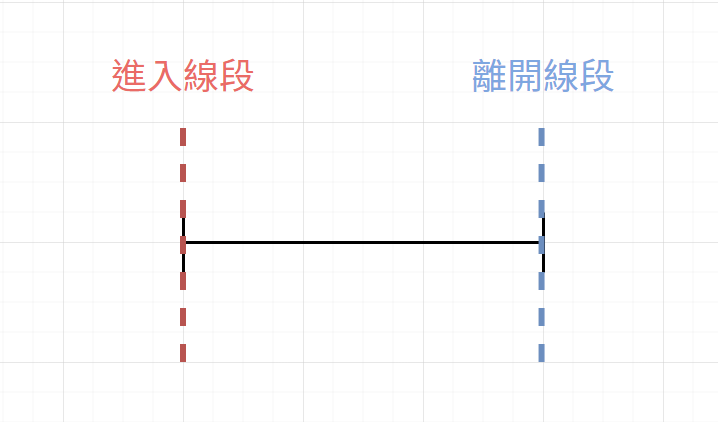
\includegraphics[scale=0.4]{images/sweep_line_2.png}
        \end{center}
    \end{frame}
    
    \begin{frame}{線段覆蓋長度}
        實作細節:
        \begin{itemize}
            \item 用 pair 去儲存每條線段的左界與右界
            \item  $\{l,1\}$ 表示在 $l$ 的位置進入線段,$\{r+1,-1\}$ 表示在 $r+1$ 的位置離開了線段
            \item 用一個數字 $a$ 維護目前掃描線經過了幾個線段,只要去維護有幾個位置 $a > 0$ 即可
        \end{itemize}
    \end{frame}
    
    \begin{frame}{下一個例題}
        \begin{block}{\href{https://atcoder.jp/contests/abc188/tasks/abc188_d}{ABC188D - Snuke Prime}}
            有一間公司推出了訂閱制的服務,訂閱後可以免費使用任何的 app,訂閱這個服務每天需要付 $C$ 塊錢,隨時都可以訂閱和解除。現在,你有 $n$ 個需要使用的 app,你知道每個 app 你會需要使用的時間是第 $a_i$ 天到第 $b_i$ 天,在沒有訂閱的情況下,每天會需要付 $c_i$ 的錢。請問你最少會需要花多少錢? \\
            \vspace{5mm}
            範圍:
            \begin{itemize}
                \item $1 \le n \le 2 \times 10^5$
                \item $1 \le C,a_i,b_i,c_i \le 10^9$
            \end{itemize}
        \end{block}
    \end{frame}
    
    \begin{frame}{下一個例題}
        \begin{itemize}
            \item 發現到每一天只有兩種選擇,訂閱服務或者是付所有 app 的錢
            \item<2-> 因此我們只要知道每一天付 app 需要花費的錢,與 $C$ 取 min 即可
            \item<3-> 與剛剛的想法很類似,只要使用掃描線去維護一段時間內的花費,一起計算即可!
        \end{itemize}
    \end{frame}
    
    \begin{frame}{一個酷酷的例題}
        \begin{block}{\href{https://codeforces.com/edu/course/2/lesson/6/3/practice/contest/285083/problem/A}{Codeforces EDU - Get together}}
            在一條數線上,有 $n$ 個人,第 $i$ 個人站在 $a_i$ 的位置上,每個人每秒走路的速度是 $v_i$ 現在,這 $n$ 個人想要聚在同一個點,請問最少要花多少時間才能讓他們站在同一個位置 \\
            \vspace{5mm}
            範圍:
            \begin{itemize}
                \item $1 \le n \le 2 \times 10^5$
                \item $1 \le v_i \le 10^9$
                \item $-10^9 \le x \le 10^9$
            \end{itemize}
        \end{block}
    \end{frame}
    
    \begin{frame}{Get together}
        \begin{itemize}
            \item 遇到這種要找最小可以達成某件事情的題目時
            \item 考慮進行二分搜
            \item<2-> 因此,現在題目轉換為,要檢查在某個時間點 $t$ 的時候,每個人是否有辦法聚在一起
            \item<3-> 在時間點 $t$ 時,每個人可以走到的位置會是 $[a_i-v_it,a_i+v_it]$
            \item<4-> 現在問題就被我們轉換成,有 $n$ 個線段,而這 $n$ 個線段是否有交集
        \end{itemize}
    \end{frame}
    
    \begin{frame}{Get together}
        \begin{itemize}
            \item 要如何檢查線段是否有交集呢?
            \item<2-> 掃描線?
            \item<3-> 其實根本不用,只要左界的最大值小於右界的最小值就好了!
        \end{itemize}
        
        \begin{center}
            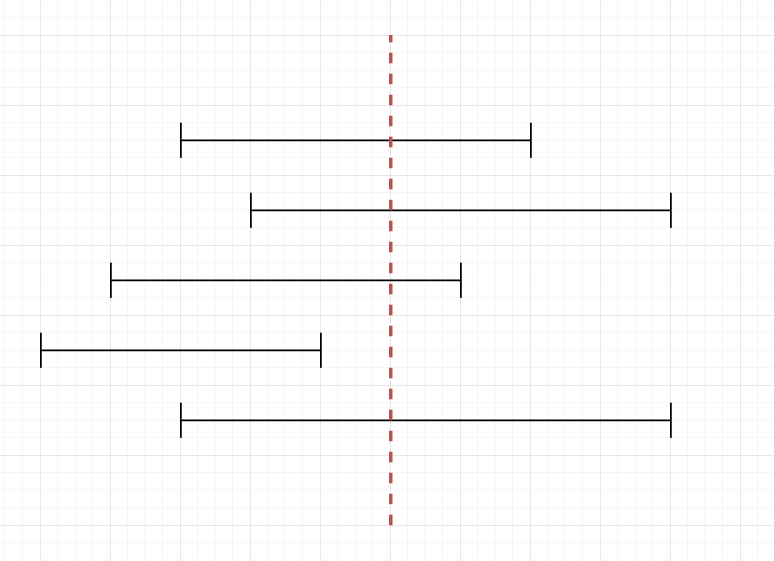
\includegraphics[scale=0.35]{images/sweep_line_3.png}
        \end{center}
    \end{frame}
    
    \begin{frame}{其他應用}
        \begin{itemize}
            \item 最近點對 (使用 set 的做法)
            \item 矩形覆蓋面積 (搭配資結)
            \item 線段交點數量 (搭配資結)
            \item 極角掃描線 (計算幾何)
            \item 還有更多...
        \end{itemize}
    \end{frame}
    
    \section{前綴和 \& 差分}
    
    \begin{frame}{一個簡單的小例子}
        \begin{block}{\href{https://cses.fi/problemset/task/1646}{CSES - Static Range Sum Queries}}
            給你一個 $n$ 項的陣列,每次詢問 $[l,r]$ 之間所有數字的總和。 \\
            \vspace{5mm}
            範圍: $1 \le n,q \le 10^5$
        \end{block}
        \begin{itemize}
            \item 既然想要求 $[l,r]$ 之間數字的總和,那每次都直接跑過所有數字不就好了?
            \item<2-> 然後這樣子的複雜度會是 $O(nq)$,會 TLE 欸?
        \end{itemize}
    \end{frame}
    
    \begin{frame}{一個簡單的小例子}
        \begin{block}{\href{https://cses.fi/problemset/task/1646}{CSES - Static Range Sum Queries}}
            給你一個 $n$ 項的陣列,每次詢問 $[l,r]$ 之間所有數字的總和。 \\
            \vspace{5mm}
            範圍: $1 \le n,q \le 10^5$
        \end{block}
        \begin{itemize}
            \item 仔細想一下,我們其實是要求一段連續數字的總和,真的需要每次都跑過一次嗎?
            \item<2-> 而這時,我們就會用到所謂的前綴和!
        \end{itemize}
    \end{frame}
    
    \begin{frame}{前綴和}
        \begin{itemize}
            \item 定義 $\texttt{pref[i]} = \sum_{j=1}^i a_i$,也就是 $[1,i]$ 所有數字的總和
            \item 則我們會發現,其實 $[l,r]$ 可以用 $[1,r]$ 減去 $[1,l-1]$ 來得到
            \item 因此只要我們跑過一次整個陣列,就可以在 $O(1)$ 的時間,得到任意區間的總和了
        \end{itemize}
        \begin{center}
            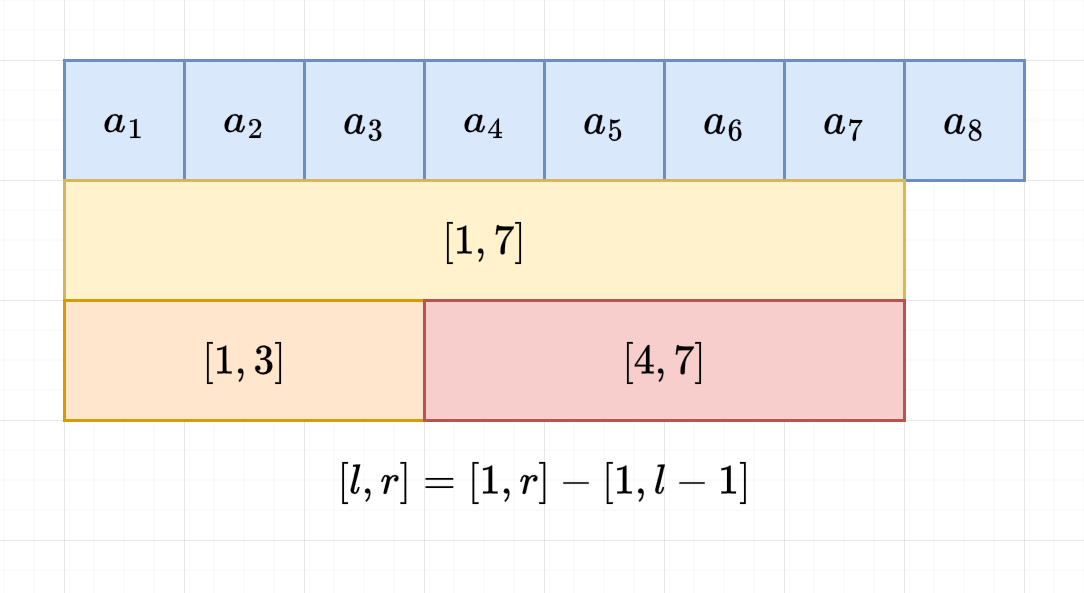
\includegraphics[scale=0.25]{images/prefix_sum.png}
        \end{center}
    \end{frame}
    
    \begin{frame}{下一個小例子}
        \begin{block}{\href{https://www.hackerrank.com/challenges/crush/problem}{HackerRank - Array Manipulation}}
            給你一個 $n$ 項的陣列,一開始每個數字都是 $0$,每次對 $[l_i,r_i]$ 的數字加上 $v_i$。在做完所有操作之後,輸出整個陣列最大的數字。 \\
            \vspace{5mm}
            範圍: 
            \begin{itemize}
                \item $1 \le n \le 10^7$
                \item $1 \le m \le 2 \times 10^5$
            \end{itemize}
        \end{block}
        \begin{itemize}
            \item<2-> 如果剛剛有認真聽課,應該會發現這題其實如果我們把區間加值想成線段
            \item<2-> 使用掃描線其實就可以計算出每個位置在操作完的數字了!
            \item<3-> 不過事實上,我們在做的這件事情,其實概念上是所謂的「差分」
        \end{itemize}
    \end{frame}
    
    \begin{frame}{差分}
        \begin{itemize}
            \item 注意到當我們對一段連續區間 $[l,r]$ 進行加值時
            \item 對於這個區間內,兩兩相鄰的數字之間有一個東西不會改變
            \item 而那就是兩兩之間的\textbf{差}
        \end{itemize}
    \end{frame}
    
    \begin{frame}{差分}
        \begin{itemize}
            \item 對於原本的陣列 $a_1,a_2,\cdots,a_n$,我們另外開一個陣列 $b$
            \item 令 $b_i = a_i - a_{i-1}$,我們稱 $b$ 為 $a$ 的「差分陣列」
            \item<2-> 當我們對一整個區間進行加值時,其實只會改變 $b_l$ 和 $b_{r+1}$
            \item<2-> 分別對應的操作是 $b_l := b_l+v, \ b_{r+1} := b_{r+1}-v$
            \item<2-> 因此每個操作我們都只需要花 $O(1)$ 的時間即可完成
            \item<3-> 在做完所有操作之後,只要對差分陣列找出前綴和即可
        \end{itemize}
    \end{frame}
    
    \begin{frame}{前綴和與差分之間的關係}
        \begin{itemize}
            \item 在很多時候,我們常常會利用到前綴和與差分來幫助我們更快速地完成一些操作
            \item 這兩種操作事實上也互為反操作
            \item 因此,其實只要有兩個互為逆運算的操作 ($+/-$, $\times/\div$, $\oplus/\oplus$)都可以做類似的事
            \item 之後學到可以做動態前綴和的資料結構 BIT 的時候,也會利用到這兩種操作
        \end{itemize}
    \end{frame}
    
    \begin{frame}{變成區間加等差數列呢?}
        \begin{block}{區間加等差數列,單點查值}
            給你一個 $n$ 項的陣列,每次對 $[l_i,r_i]$ 的數字依序加上 $v_i, v_i+d_i, v_i+2d_i, \cdots$。在做完所有操作之後,輸出所有數字。 \\
            \vspace{5mm}
            範圍: 
            \begin{itemize}
                \item $1 \le n \le 10^5$
                \item $1 \le m \le 10^5$
            \end{itemize}
        \end{block}
    \end{frame}
    
    \begin{frame}{變成區間加等差數列呢?}
        \begin{itemize}
            \item 發現到每個位置被加的值會依序遞增
            \item 用一個神奇的表示方式,將目前的 $a_i := x_i \times i + y_i$
        \end{itemize}
        \begin{center}
            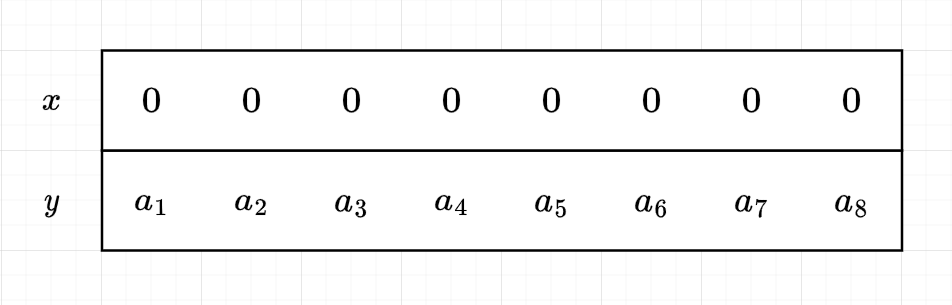
\includegraphics[scale=0.4]{images/range_add_ap.png}
        \end{center}
    \end{frame}
    
    \begin{frame}{變成區間加等差數列呢?}
        \begin{itemize}
            \item 事實上等同於對 $x_i$ 和 $y_i$ 分別做區間加值
            \item 分別維護兩個的差分即可
        \end{itemize}
        \begin{center}
            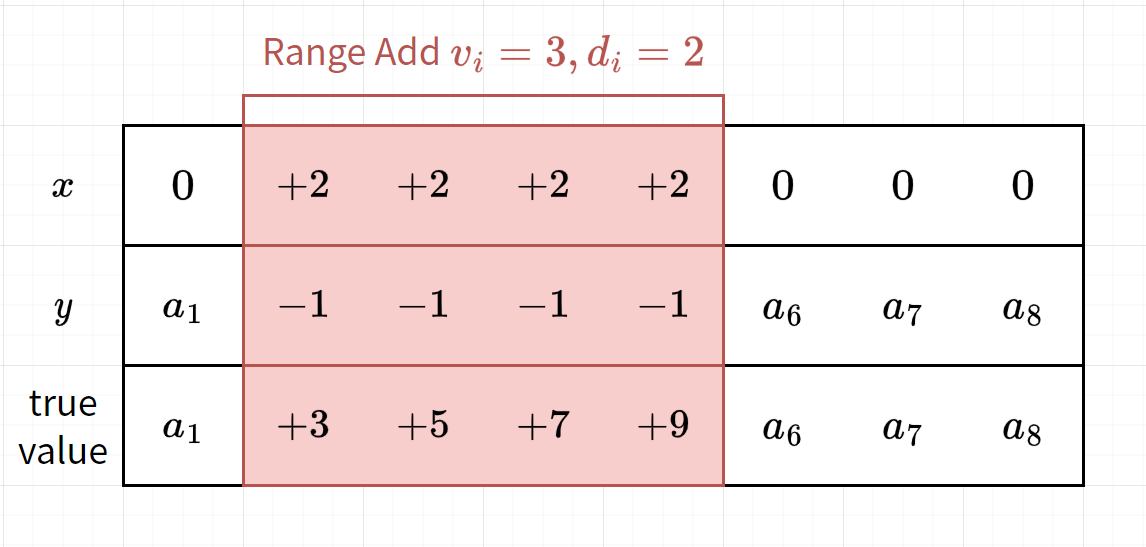
\includegraphics[scale=0.4]{images/range_add_ap_2.png}
        \end{center}
    \end{frame}
    
    \begin{frame}{變成區間加等差數列呢?}
        \begin{itemize}
            \item 我們用 \texttt{diffx[i]} 與 \texttt{diffy[i]} 來分別表示兩個的差分
            \item 對區間 $[l,r]$ 加等差數列時,等同於
                \begin{enumerate}
                    \item $\texttt{diffx[l]} := \texttt{diffx[l]} + d_i$, $\texttt{diffx[r+1]} := \texttt{diffx[r+1]} - d_i$
                    \item $\texttt{diffy[l]} := \texttt{diffy[l]} + v_i - i \times d_i$, $\texttt{diffy[r+1]} := \texttt{diffy[r+1]} - v_i + i \times d_i$
                \end{enumerate}
            \item 做完之後再一起做前綴和,找到真正的 $x_i, y_i$,就可以找到真正的 $a_i$ 了
        \end{itemize}
    \end{frame}
    
    \begin{frame}{二維前綴和}
        \begin{block}{\href{https://cses.fi/problemset/task/1652}{CSES - Forest Queries}}
            給你一個二維的表格,每個位置上可能會有種樹。接著詢問 $q$ 次,每次詢問 $(a,b)$ 和 $(c,d)$ 所夾成的矩形內有幾棵樹?
        \end{block}
    \end{frame}
    
    \begin{frame}{二維前綴和}
        \begin{itemize}
            \item 現在問題從剛剛的陣列上的詢問,變成是二維表格上的詢問了
            \item 能不能用類似的方式計算答案呢?
        \end{itemize}
        \begin{center}
            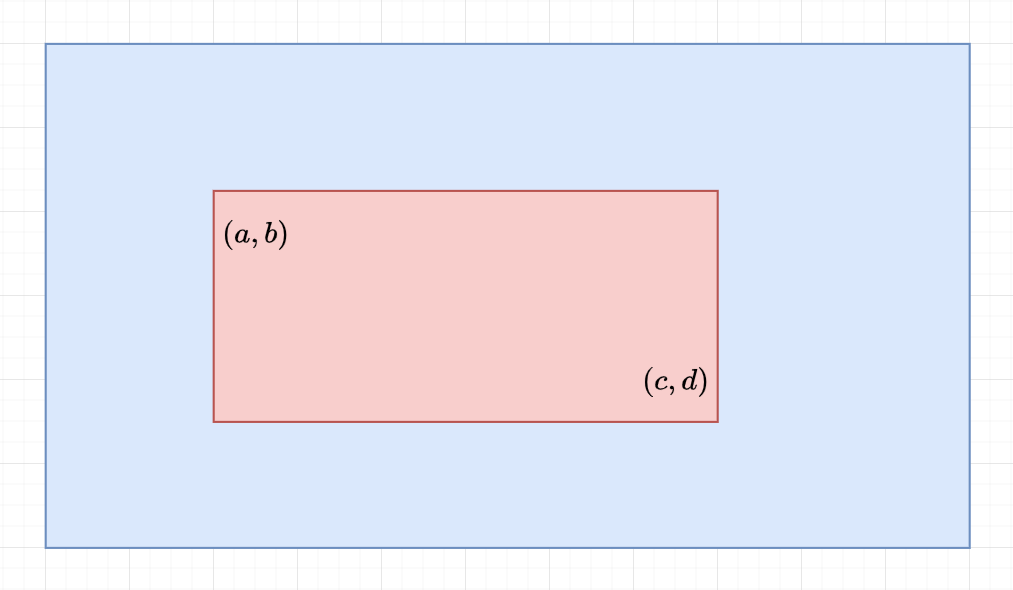
\includegraphics[scale=0.35]{images/2d_prefix_sum.png}
        \end{center}
    \end{frame}
    
    \begin{frame}{二維前綴和}
        \begin{itemize}
            \item 事實上,我們想要找的東西是 
            $$\sum_{i=a}^c \sum_{j=b}^d a_{ij}$$
            \item 現在,我們想要用前綴和的方式來快速計算這個東西
            \item<2-> 可以用 pref[x][y] 表示  
            $$\sum_{i=1}^x \sum_{j=1}^y a_{ij}$$
            \item<2-> 就可以用類似剛剛在一維陣列上的做法得到答案了
        \end{itemize}
    \end{frame}
    
    \begin{frame}{二維前綴和}
        \begin{itemize}
            \item $sum(a,b,c,d) = \texttt{pref[c][d] - pref[a-1][d] - pref[c][b-1] + pref[a-1][b-1]}$
        \end{itemize}
        \begin{center}
            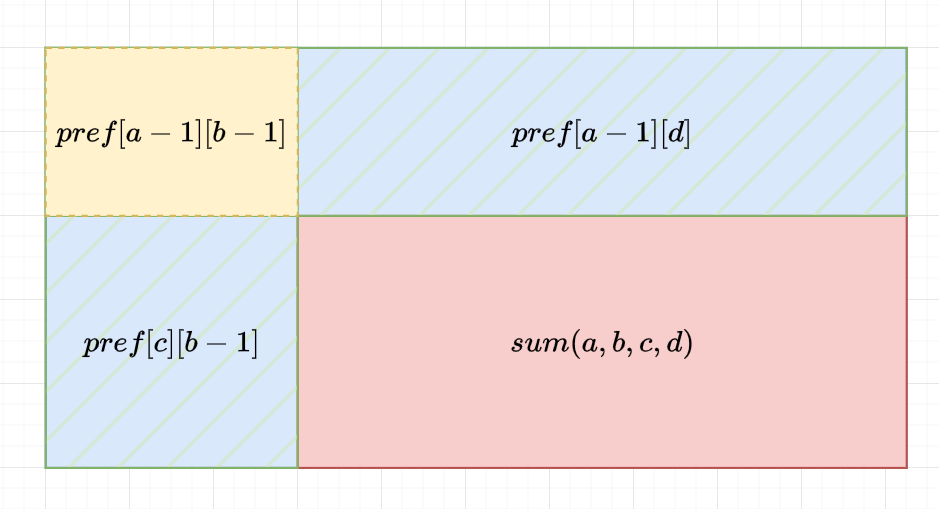
\includegraphics[scale=0.4]{images/2d_prefix_sum_2.png}
        \end{center}
    \end{frame}
    
    \begin{frame}{二維前綴和}
        \begin{itemize}
            \item 建立二維前綴和與詢問十分相似
            $$\texttt{pref[x][y] = pref[x-1][y] + pref[x][y-1] - pref[x-1][y-1]}$$
            \item 可以在 $O(nm)$ 的時間完成預處理
        \end{itemize}
    \end{frame}
    
    \begin{frame}{二維差分?}
        \begin{itemize}
            \item 既然有二維前綴和,那有沒有二維差分?
            \item 有的!作法也很類似,留給大家自己思考看看
            \item<2-> 小提示是一維的差分對 $l$ 加值等同於對後綴加值
            \item<2-> 那對二維的差分加值,會等同什麼呢?
        \end{itemize}
    \end{frame}
    
    \section{單調隊列}
    
    \begin{frame}{來看一個簡單的小例題}
        \begin{block}{\href{https://cses.fi/problemset/task/1645/}{CSES - Nearest Smaller Value}}
            給你一個 $n$ 項的序列,請找到每個元素往左邊找第一個小於這個數字的位置。
        \end{block}
        \begin{itemize}
            \item<2-> 遇到這個題目後,你可能會想要直接對每個數字往前枚舉,找到想要的答案。
            \item<2-> 不過這樣做會是 $O(n^2)$。
            \item<3-> 有沒有更好的做法呢?
        \end{itemize}
    \end{frame}
    
    \begin{frame}{來看一個簡單的小例題}
        \begin{itemize}
            \item 因此,我們要來講講單調隊列這個東西
            \item 使用一個 stack 紀錄
            \item 維護一個遞增或遞減的序列
            \item 遞增 $\rightarrow$ 第一個位置是整個陣列的最小值
            \item 遞減 $\rightarrow$ 第一個位置是整個陣列的最大值
        \end{itemize}
    \end{frame}
    
    \begin{frame}{回到原題}
        \begin{itemize}
            \item 注意到當我們從左開始往右枚舉數字時
            \item 在 $a_i$ 前面大於 $a_i$ 的數字都在後來都沒有用了
        \end{itemize}
        \begin{center}
            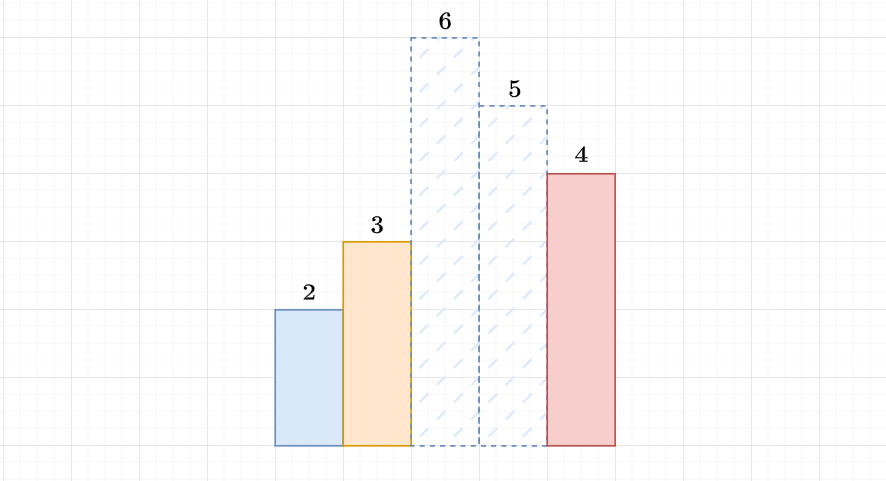
\includegraphics[scale=0.4]{images/monotonic stack.png}
        \end{center}
    \end{frame}
    
    \begin{frame}[fragile]{回到原題}
        \begin{itemize}
            \item 因此,我們根本不用在每一次遇到新數字都去往前找
            \item 需要的資訊都存在 stack 上面了
            \item 時間複雜度: $O(n)$
            \item 參考程式碼:
        \end{itemize}
        \begin{lstlisting}[language=C++,basicstyle=\ttfamily\tiny]
    stack<int> st;
 
    for(int i = 1;i <= n;i++){
        while(!st.empty() && arr[st.top()] >= arr[i]){
            st.pop();
        }
        if(!st.empty()) ans[i] = st.top();
        st.push(i);
    }
        \end{lstlisting}
    \end{frame}
    \begin{frame}{固定長度區間極值}
        \begin{block}{\href{https://zerojudge.tw/ShowProblem?problemid=a146}{Sliding Maximum/Minimum (Zerojudge a146)}}
            你有一個長度為 $n$ 的陣列 $a_1, \dots, a_n$,請找出所有長度為 $k$ 的子陣列的最大和最小值。 \\
            \vspace{5mm}
            測資範圍: $n \le 10^6$
        \end{block}
        \begin{itemize}
          \item<2-> 既然我們剛剛講到了單調隊列的概念,我們來想想這題的做法吧!
        \end{itemize}
    \end{frame}
    
    \begin{frame}{固定長度區間極值}
        \begin{itemize}
            \item 避免有人不理解剛剛題目的意思,這裡放個圖進行說明
        \end{itemize}
        \begin{center}
            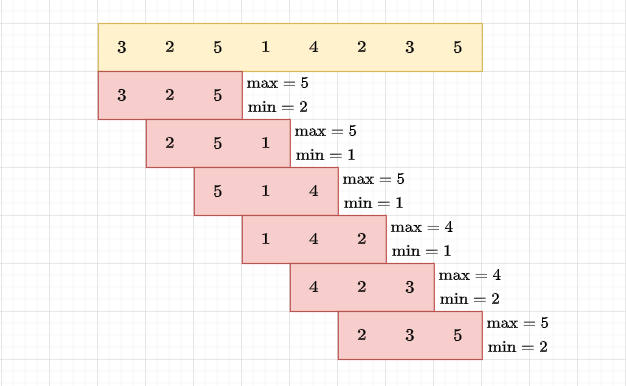
\includegraphics[scale=0.6]{images/sliding_max_min.png}
        \end{center}
    \end{frame}
    
    \begin{frame}[fragile]{固定長度區間極值}
        \begin{itemize}
            \item 現在,我們想一個簡單一點的問題,我們對前綴找出維護最大值的單調隊列試試
        \end{itemize}
        \begin{center}
            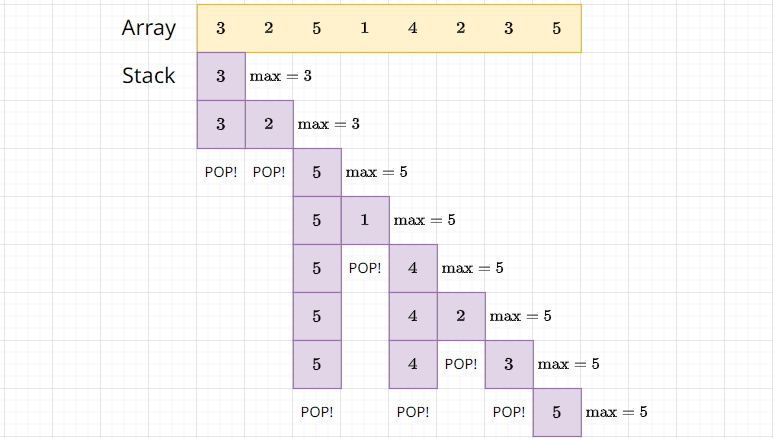
\includegraphics[scale=0.45]{images/prefix_max.png}
        \end{center}
    \end{frame}
    
    \begin{frame}[fragile]{固定長度區間極值}
        \begin{itemize}
            \item 用一樣的做法,不過長度超過 $k$ 的也跟著 POP 掉!
        \end{itemize}
        \begin{center}
            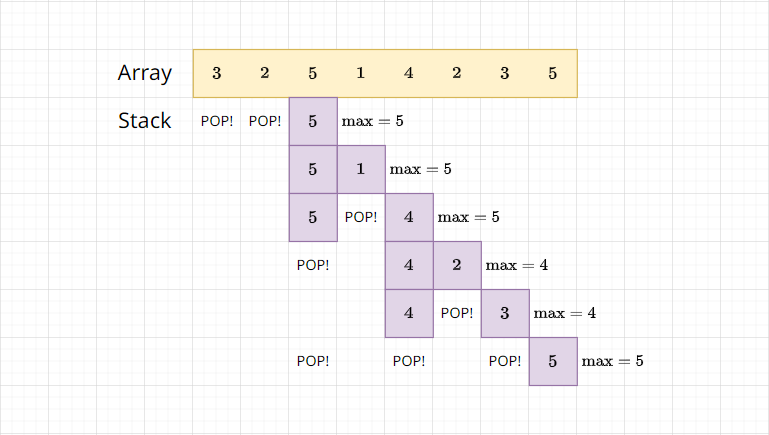
\includegraphics[scale=0.45]{images/sliding_max.png}
        \end{center}
    \end{frame}
    
    \begin{frame}[fragile]{固定長度區間極值}
        一些小小的實作細節
        \begin{itemize}
            \item 為了只維護長度在 $k$ 以內的 window,我們會在 deque 上面存 index
            \item 維護最大值 $\rightarrow$ 前面有比較小的就 pop 掉
            \item 維護最小值 $\rightarrow$ 前面有比較大的就 pop 掉
            \item 詳細的話,我們等等來講實際的程式碼
            \item 同樣的東西會在 DP II 遇到,大家要搞懂這邊喔!
        \end{itemize}
    \end{frame}
    
    \begin{frame}[fragile]{參考程式碼}
        \begin{lstlisting}[language=C++,basicstyle=\ttfamily \small]
    for(int i = 0;i < n;i++){
        //MIN
        while(!mn.empty() && i-mn.front() >= k)
            mn.pop_front();
        while(!mn.empty() && arr[mn.back()] >= arr[i])
            mn.pop_back();
        mn.push_back(i);
        if(i >= k-1) ansMN.push_back(arr[mn.front()]);
        //MAX
        while(!mx.empty() && i-mx.front() >= k)
            mx.pop_front();
        while(!mx.empty() && arr[mx.back()] <= arr[i])
            mx.pop_back();
        mx.push_back(i);
        if(i >= k-1) ansMX.push_back(arr[mx.front()]);
    }
        \end{lstlisting}
    \end{frame}
    
    \begin{frame}{經典例題 - 最大長方形面積}
        \begin{block}{\href{https://cses.fi/problemset/task/1142}{CSES - Advertisement}}
            現在有 $n$ 個寬為 $1$,長為 $a_i$ 的長條排成一列,請找到最大的長方形面積是多少
        \end{block}
        \begin{center}
            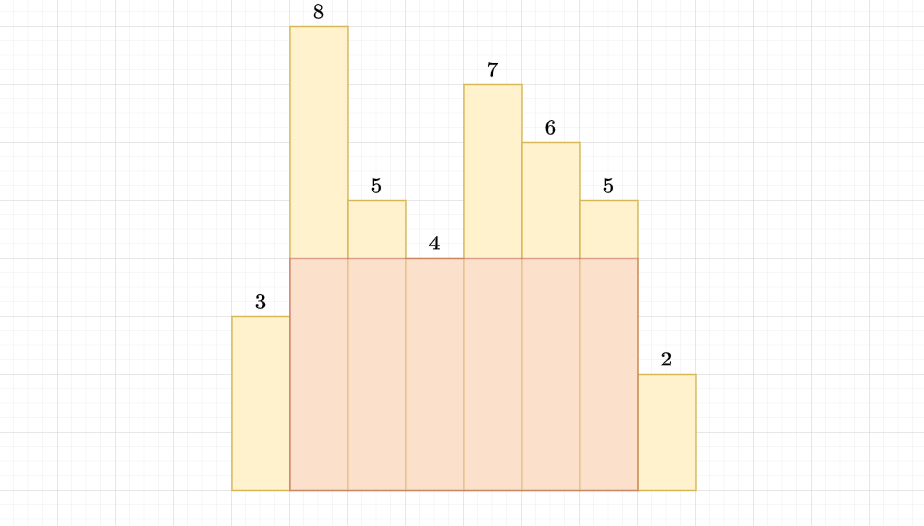
\includegraphics[scale=0.4]{images/CSES_Advertisement.png}
        \end{center}
    \end{frame}
    
    \begin{frame}{經典例題 - 最大長方形面積}
        \begin{itemize}
            \item 有沒有什麼想法呢?
            \item<2-> 最簡單的方式是枚舉一整個區間 $[l,r]$,而答案會是 $(r-l+1) \min\{a_l,\cdots,a_r\}$ 的最大值
            \item<3-> 不過這樣做太慢了!
        \end{itemize}
    \end{frame}
    
    \begin{frame}{經典例題 - 最大長方形面積}
        \begin{itemize}
            \item 注意到我們可以換一個思路
            \item 對每個 $a_i$,往左往右找最遠到哪個位置,$a_j$ 都會大於等於 $a_i$
            \item 我們用 l[i] 與 r[i] 表示,那答案其實就是 $\displaystyle \max_{i=1}^n (r[i]-l[i]+1)a_i$
        \end{itemize}
        \begin{center}
            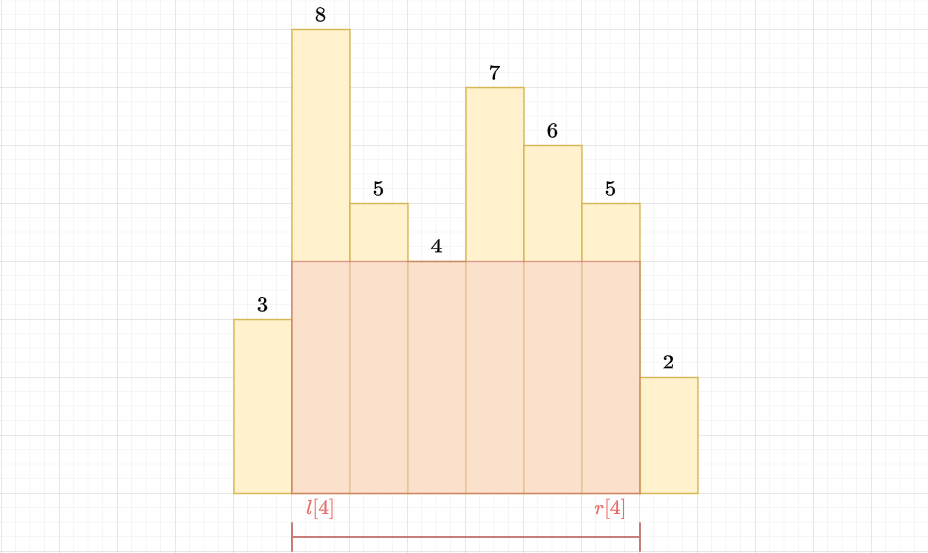
\includegraphics[scale=0.3]{images/CSES_Advertisement_2.png}
        \end{center}
    \end{frame}
    
    \begin{frame}{經典例題 - 最大長方形面積}
        \begin{itemize}
            \item 怎麼計算 l[i] 和 r[i] 呢?
            \item 其實就是剛剛講過的第一個小於 $x$ 的位置,但從左右都各做一次!
            \item 時間複雜度: $O(n)$
        \end{itemize}
    \end{frame}
    
    \begin{frame}{經典例題 - 最大全 0 矩形}
        \begin{block}{\href{https://cses.fi/problemset/task/1147}{CSES - Maximum Building I}}
            給你一張網格圖,每個位置可能會種樹,也可能不會種樹。你現在要建造一個長方形的房子,但有種樹的格子上不能蓋房子,請問這個房子最大可以是多少?
        \end{block}
        Hint: 這題其實就是剛剛那題,留給大家當作練習
    \end{frame}
    
    \section{補充: 模運算}
    
    \begin{frame}{模運算}
        \begin{itemize}
            \item 這邊的內容會在數學的時候講述更多
            \item 不過因為這件事還滿重要的,我們在此先講一下模運算
            \item 但這裡會先用比較沒那麼嚴謹的方式進行說明
        \end{itemize}
    \end{frame}
    
    \begin{frame}{模運算}
        \begin{itemize}
            \item 你可能常常會在題目上遇到這樣的要求
            \item 「由於答案可能會很大,請輸出 $\bmod \ 10^9+7$ 後的結果」
            \item 這邊的 $\bmod$ 究竟是什麼意思呢?
        \end{itemize}
    \end{frame}
    
    \begin{frame}{模運算}
        \setbeamercolor{block title}{use=structure,bg=green!50!black}
        \begin{block}{模運算 (Modulo Operation)}
            定義 $a \bmod b = r$,表示你可以找到一個 $q \in \mathbb{Z}$,使得 $a = bq+r$,而 $0 \le r < b$ 
            \begin{itemize}
                \item 等同於 C++ 當中的 \texttt{\%} 所做的事情
                \item 事實上,C++ 的 \texttt{\%} 做的事情就是這個,不同的點在於可能會有負數
                \item C++ 的 \texttt{\%} 定義為 $a \ \% \ b = a-b \times \Big \lfloor \frac{a}{b} \Big \rfloor$
                \item 由於 int 和 long long 都有固定的範圍,我們會利用 mod 來避免超出範圍
            \end{itemize}
        \end{block}
    \end{frame}
    
    \begin{frame}{模運算}
        \begin{alertblock}{模運算的性質}
            \begin{enumerate}
                \item $(a + b) \bmod n = ((a \bmod n) + (b \bmod n))\bmod n$
                \item $ab \bmod n = (a \bmod n) (b \bmod n) \bmod n$
                \item $\dfrac{a}{b} \bmod n \ne \dfrac{a \bmod n}{b \bmod n}$
            \end{enumerate}
        \end{alertblock}
        \begin{itemize}
            \item 前兩點告訴我們,其實在進行加減和乘的時候,不管有沒有 mod 都是一樣的
            \item 不過第三點是錯的\textbf{超級重要},這點絕對要記住
            \item 如何在有 mod 的時候進行除法,會在之後的數學課時講到
        \end{itemize}
    \end{frame}
    
    \begin{frame}{模運算性質證明 (一)}
        令 $a = k_1n + r_1, \ b = k_2n + r_2$,而 $k_1,k_2 \in \mathbb{Z}$ and $0 \le r_1,r_2 < n$。根據 mod 的定義, $r_1 = a \bmod n, \ r_2 = b \mod n$.
        \begin{align*}
        (a+b) \bmod n &= (k_1n+r_1 + k_2n+r_2) \bmod n \\
                      &= (n(k_1+k_2) + r_1 + r_2) \bmod n \\
                      &= (r_1 + r_2) \bmod n \\
                      &= (a \bmod n) + (b \bmod n) \bmod n
        \end{align*}
        因此,我們證明了 $(a + b) \bmod n = ((a \bmod n) + (b \bmod n))\bmod n$.
    \end{frame}
    
    \begin{frame}{模運算性質證明 (二)}
        令 $a = k_1n + r_1, \ b = k_2n + r_2$,而 $k_1,k_2 \in \mathbb{Z}$ and $0 \le r_1,r_2 < n$。根據 mod 的定義, $r_1 = a \bmod n, \ r_2 = b \mod n$.
        \begin{align*}
        ab \bmod n  &= (k_1n+r_1)(k_2n+r_2) \bmod n \\
                    &= (k_1k_2n^2 + k_1r_2n + k_2r_1n + r_1r_2) \bmod n \\
                    &= (n(k_1k_2n + k_1r_2 + k_2r_1) + r_1r_2) \bmod n \\
                    &= r_1r_2\bmod n \\
                    &= (a \bmod n)(b \bmod n) \bmod n
        \end{align*}
        因此,我們證明了 $ab \bmod n = (a \bmod n)(b \bmod n) \bmod n$.
    \end{frame}
    
    \begin{frame}{模運算結論}
        \begin{itemize}
            \item 不過講了那麼多,相信有些人還是不能理解剛剛所講的東西
            \item 但沒關係,只要記得不論是加減乘,先 mod 或後 mod 都是一樣的
        \end{itemize}
    \end{frame}
    
    \begin{frame}{模運算小練習}
        我們來做點小練習吧!
        \begin{block}{用 C++ 計算以下數值}
            \begin{enumerate}
                \item $100000 \times 99999 \bmod 13$
                \item $2^{100} \bmod 10^9+7$
                \item $(-4) \times 1234567890 \bmod 998244353$
                \item 費氏數列 ($1,1,2,3,5,8,...$) 第 $100$ 項 $\bmod \ 10^9+7$
                \item 一個奇怪的遞迴數列第 $100$ 項 $\bmod \ 998244353$
                $$
                f(n) = \begin{cases}
                    1 & \text{if } n \le 1, \\
                    f(n-1)f(n-2) - 2f(n-1) - 3f(n-2) & \text{otherwise} \\
                \end{cases}
                $$
            \end{enumerate}
        \end{block}
    \end{frame}
    
    \begin{frame}{模運算小練習}
        \begin{block}{練習題的答案}
            \begin{enumerate}
                \item 12
                \item 976371285
                \item 52950205
                \item 782204094
                \item 901665516
            \end{enumerate}
        \end{block}
    \end{frame}
    
\end{document}